\section{Results}

\subsection{Quantitative Results}
We evaluate Q-learning (QL), model-based RL (MBRL) and Floyd-Warshall
Reinforcement Learning (FWRL) on two metrics in two different environments. The
two metrics we use are Latency Ratio and average reward per episode. The Latency
ratio metric was introduced in \citet{MiPaViICLR2017}, which is defined as the
ratio of time taken to reach the goal for the first to time to the average time
taken to hit the goal thereafter. The Latency ratio thus measures the ratio of
exploration time for first time finding the goal to the average exploitation
time to reach the goal. Hence, higher latency ratio is better.
Fig~\ref{fig:ql-fw-grid-world-results} and
Fig~\ref{fig:ql-fw-windy-world-results} show the results.

\begin{figure}%
    \begin{subfigure}
        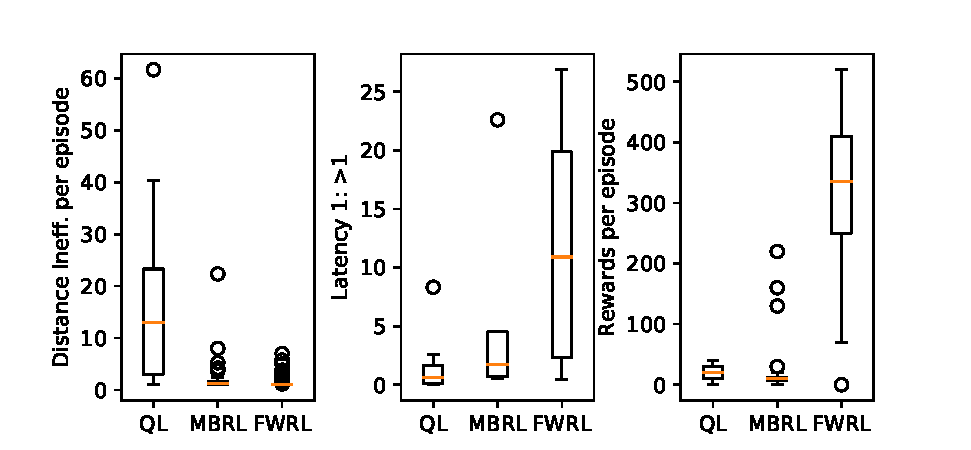
\includegraphics[width=\columnwidth]{./media/metrics-grid-world.pdf}{a}
        \caption{Results on grid world. FWRL beats Q-Learning
        consistently. Lower is better for Distance-Inefficiency. Higher
        is better for reward per episode. }
    \end{subfigure}
    \begin{subfigure}
        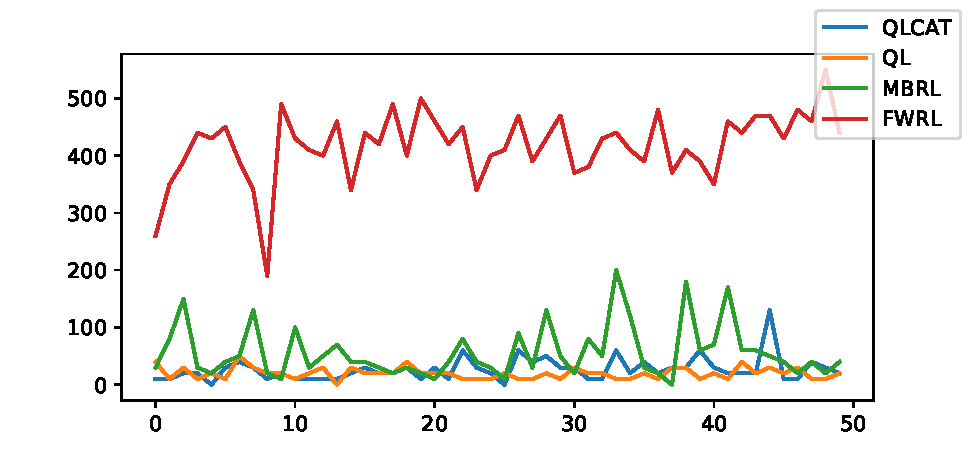
\includegraphics[width=\columnwidth]{./media/rewards-metrics-grid-world.pdf}{b}
        \caption{Reward curves on grid world. FWRL reward climbs much
        faster than all other baselines showcasing the improved \emph{sample
        efficiency} of the algorithm.}
    \end{subfigure}
    \label{fig:ql-fw-grid-world-results}%
\end{figure}


\begin{figure}
    \begin{subfigure}
        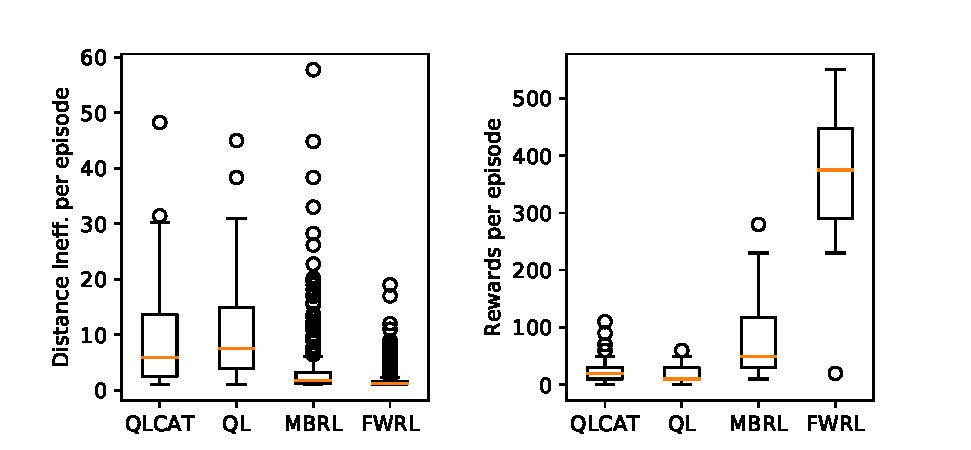
\includegraphics[width=\columnwidth]{./media/metrics-windy-world.pdf}
        \caption{Results on windy world. FWRL beats Q-Learning
        consistently. Lower is better for Distance-Inefficiency. Higher
        is better for reward per episode. }
    \end{subfigure}
    \begin{subfigure}
        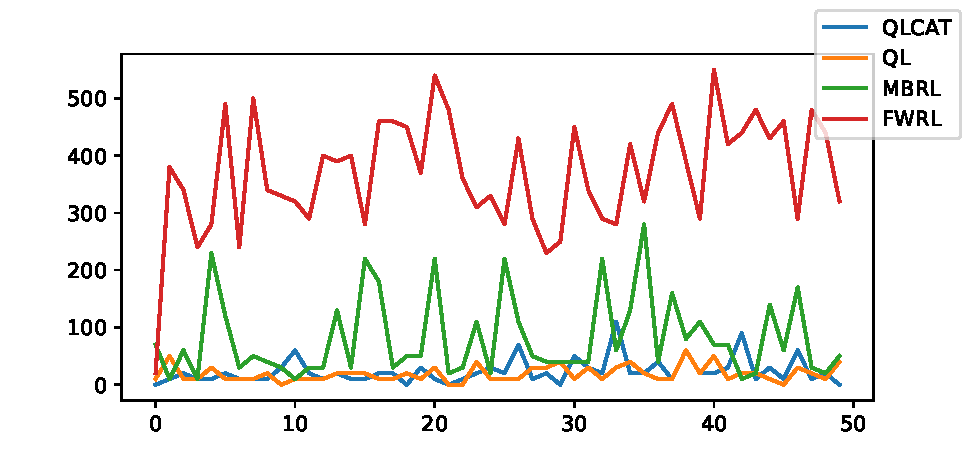
\includegraphics[width=\columnwidth]{./media/rewards-metrics-windy-world.pdf}
        \caption{Reward curves on windy world. FWRL reward climbs much
        faster than all other baselines showcasing the improved \emph{sample
        efficiency} of the algorithm.}
    \end{subfigure}
    \label{fig:ql-fw-windy-world-results}%
\end{figure}


\subsection{Qualitative Results}
